\section{The XG-PON Module for NS-3} \label{section_design}


%With the release of XG-PON standard, XG-PON product development
%will be speeded up, %XG-PON network deployment will come soon,
%and for this reason it becomes important  to study the performance issues
%arising with the deployment of XG-PON. %Considering that XG-PON is still in its early stage,
%To study these issues, an XG-PON module has been developed by us
%for NS-3, a state of the art open-source network simulator. The

This section describes in detail the XG-PON module we have
developed for NS-3. Our aim is to provide a standard compliant,
configurable, and extensible module that can simulate XG-PON with
reasonable speed and can support a wide range of research topics.

%Although NS-3 has provided many useful features, such as its novel attribute system for configuring simulation parameters, there are still many challenges to be solved and many tradeoffs to be made.
%In this section, we will present the design and implementation details of this XG-PON module. The challenges and tradeoffs are also discussed in the course.



\subsection{Overview of the XG-PON Module} \label{subsection_xgponoverview}

%In the following paragraphs, we will present one overview of this XG-PON module and justify the important simplifications.


\begin{figure}[!htbp]
\begin{center}
\includegraphics[width=0.9\textwidth]{images/design_xgpon_overall}
\end{center}
\vspace{-0.1in}
\caption{The Reference XG-PON Simulation}
\label{fig_xgpon_reference_simulation}
\end{figure}


Figure \ref{fig_xgpon_reference_simulation} illustrates a typical
simulation that uses this module and NS-3 to study the performance
issues arising with XG-PON. The OLT is simulated as a node that
has one \emph{XgponOltNetDevice} and another network device, such
as PointToPointNetDevice, to connect to an external network. The
ONU is simulated as a node with one \emph{XgponOnuNetDevice} and
other network devices (Ethernet, WiFi, WiMAX, LTE, etc.) for
connecting user equipments to the ONU. Thanks to NS-3, network
devices of a node can be configured and we can study different
deployment scenarios of XG-PON easily. Although XG-PON is proposed
to carry layer-2 frames of various network technologies (Ethernet,
ATM, etc.), our XG-PON module interacts directly with the IP layer
and IP packets are the SDUs. This is reasonable since we focus on
FTTx networks connected to the Internet.






The OLT and ONUs are attached to \emph{XgponChannel} that
simulates the optical distribution network (ODN) of XG-PON. As
illustrated in Figure \ref{fig_lrpon}, this ODN is a quite complex
tree composed by optical fibers, splitters/jointers, and REs. To
produce trustworthy simulation results, it is highly desirable to
simulate all details. However, XG-PON is a high speed network with
a very complex standard. In this module, many aspects have been
simplified for reducing the development workload and speeding up
the simulation speed.

Specifically, our XgponChannel just simulates $d_{max}$, i.e., the
logic one-way delay of the channel that is determined by the
maximal propagation delay of ODN and various processing delay.
$d_{max}$ can be configured through the attribute system of NS-3.
For a downstream frame from the OLT, XgponChannel will pass this
frame to each ONU after waiting for $d$, i.e., the corresponding
one-way propagation delay between the OLT and this ONU. Note that
for avoiding unnecessary data copy, XgponChannel passes the
smart-pointer of this frame to each ONU which will just copy and
process the data for itself\footnote{In the future, this feature
will be revised to support parallel simulation in which ONUs are
simulated on different CPUs of a cluster.}. As for an upstream PHY
burst, it will be postponed for the corresponding propagation
delay, but XgponChannel will pass it to the OLT only. The
equalization delay is considered by ONU when it schedules to
produce the upstream burst based on $BW_{map}$ from the OLT.


This means that although the difference of propagation delay among
ONUs is simulated, the propagation of optical signals (fiber,
splitter, etc.) is not simulated by the XgponChannel. This design
is reasonable since the targeted research topics are related with
MAC and upper layers. Through these simplifications, simulation
speed can also be significantly improved. Otherwise, many events
must be scheduled to pass a downstream XGTC frame to ONUs if
fibers and splitters are considered. It is also very CPU-intensive
to calculate the optical signal strength for each downstream frame
when it arrives to each ONU.


In the following subsection, we will present how the XG-PON
protocol stack is simulated. More specifically, we will identify
its functional blocks, followed by the design and implementation
details.




\subsection{XG-PON Functional Blocks}

Since we are interested in the performance of a running network,
the functional blocks of XG-PON are identified below through
explaining the data transmission paths in both downstream and
upstream directions.

\subsubsection{Downstream Traffic on OLT Side}

As shown in Figure \ref{fig_xgpon_functionblock}, when one SDU is
received from the upper layer, it will first be mapped to the
corresponding connection (XGEM Port) based on the destination IP
address and put into the queue for transmitting in the future.
Thus, there must be one algorithm for mapping the IP address to a
XGEM Port-Id.


\begin{figure}[!htbp]
\begin{center}
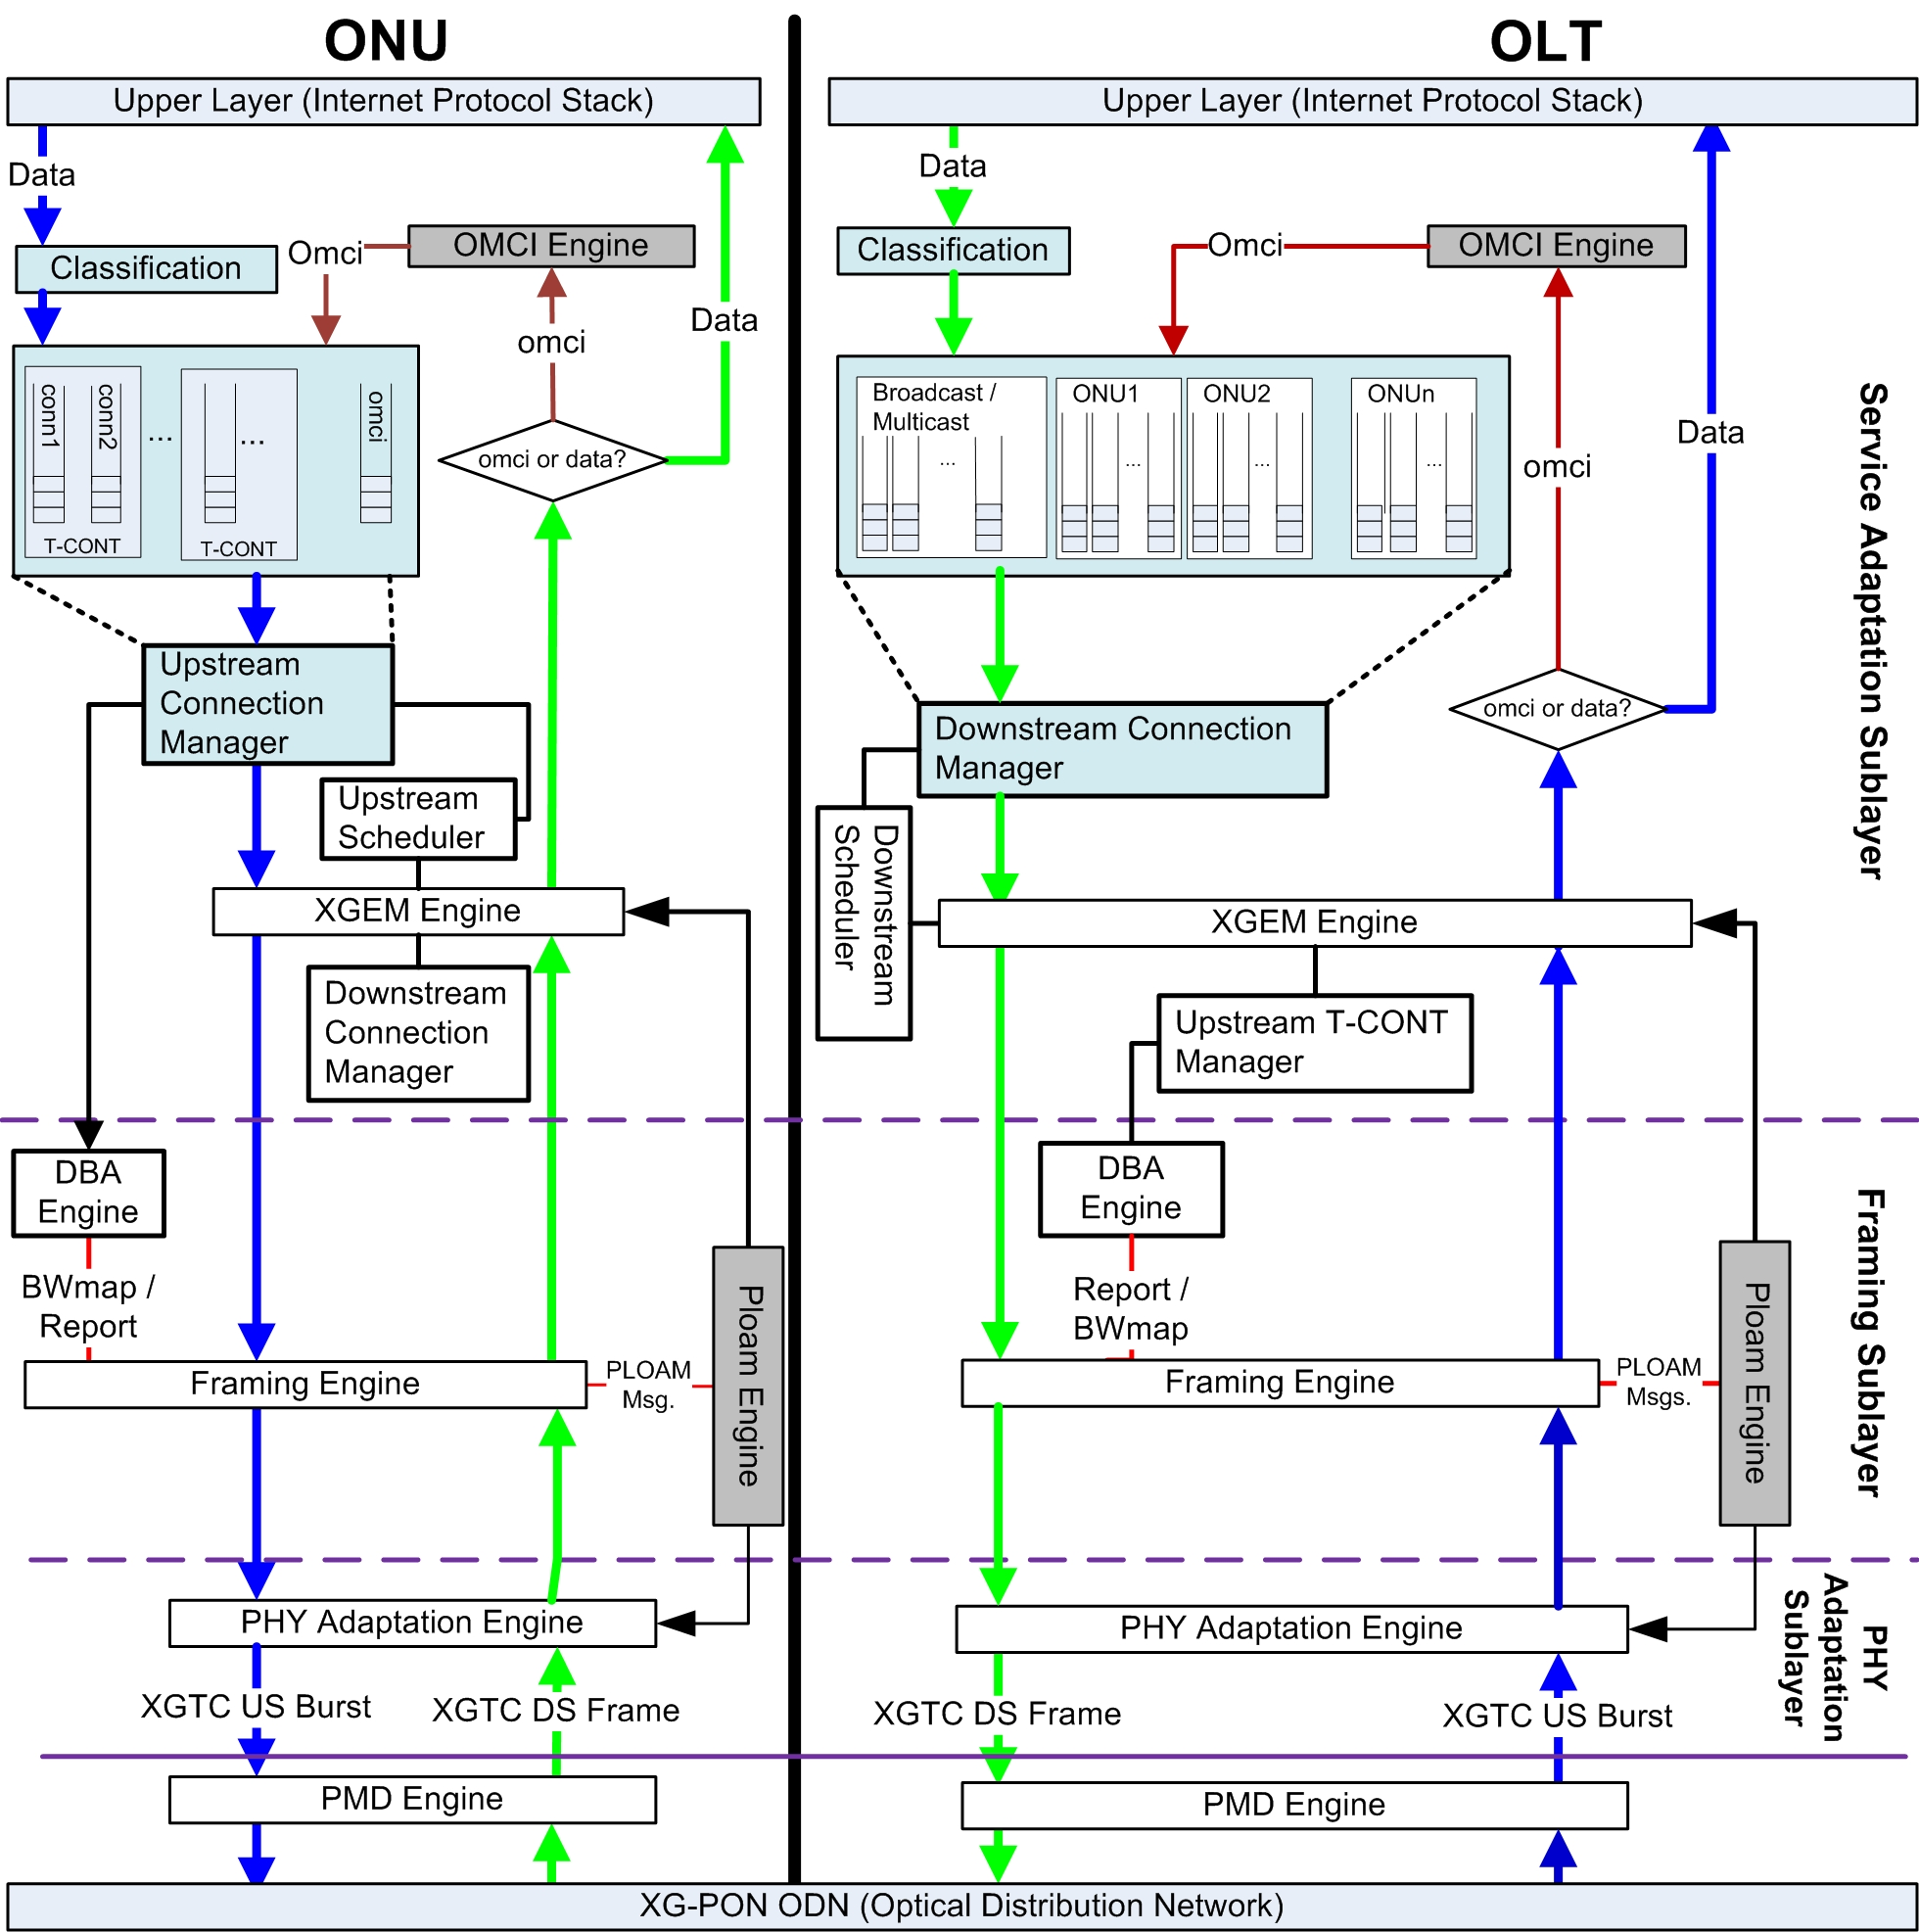
\includegraphics[width=0.9\textwidth]{images/design_function_block}
\end{center}
\vspace{-0.1in}
\caption{Function Block Diagram of XG-PON}
\label{fig_xgpon_functionblock}
\end{figure}

Since the OLT needs to broadcast the downstream XGTC frames every
125 $\mu$s, it will periodically ask the OLT's \emph{Framing
Engine} to generate a XGTC frame. This engine will first generate
an XGTC header since the available space for data in the frame
depends on the size of the XGTC header.

For the payload of a downstream XGTC frame, the Framing Engine
resorts to the \emph{XGEM Engine} to get an XGTC payload. This
payload is comprised of concatenated XGEM frames that occupy all
the available space. As for the SDUs to be encapsulated and
transmitted, the XGEM Engine lets the \emph{Downstream Scheduler}
decide the connections to be served. This scheduler makes
decisions based on \emph{Downstream Connection Manager} which
knows queue length, QoS parameters, and service history of each
downstream connection. When carrying out encapsulation,
fragmentation will be carried out by XGEM Engine if one SDU is too
long for the current transmission opportunity. XGEM Engine is also
responsible to encrypt these SDUs to avoid eavesdropping. The keys
used for data encryption are negotiated through PLOAM messages and
are maintained by \emph{Ploam Engine}.

To construct the XGTC header of the frame, the \emph{DBA Engine}
is used to generate BW$_{map}$ that tells ONUs how to share the
upstream wavelength. DBA Engine makes decisions based on queue
occupancy reports, QoS parameters, and service history of T-CONTs.
As for the PLOAM messages in the header, they are generated by
Ploam Engine.

The downstream frame is sent to the ODN after passing through
\emph{PHY Adaptation Engine} and \emph{PMD Engine}.


\subsubsection{Downstream Traffic on ONU Side}

When a downstream PHY frame arrives to one ONU, it will pass
through PMD Engine and PHY Adaptation Engine which will remove the
physical-layer overhead. The Framing Engine is then responsible to
parse the resulting downstream XGTC frame.

The PLOAM messages from the XGTC header will be given to the Ploam
Engine, which will process the messages related with this ONU. The
DBA Engine is responsible to process BW$_{map}$ in the header,
i.e., schedule its upstream XGTC bursts if required by this
BW$_{map}$.

As for the payload, the XGEM frames are passed to XGEM Engine.
Based on the list of its connections maintained by Downstream
Connection Manager, the XGEM frames for this ONU are first
extracted. XGEM Engine then carries out decapsulation, decryption,
and reassembly (if needed)\footnote{For each downstream
connection, the Downstream Connection Manager at the ONU should
hold the segments that have been received for carrying out
reassembly when the remaining segments are received.}. The
received SDUs are then sent to the upper layer.



\subsubsection{Upstream Traffic on ONU Side}

As illustrated in Figure \ref{fig_xgpon_functionblock}, when a IP
packet is received at the ONU, based on the source IP address,
it is first mapped the corresponding upstream connection
that are organized by \emph{Upstream Connection Manager}.
The packet is then put into the corresponding queue for
transmitting in the future.

When it is the time to transmit one upstream XGTC burst (scheduled
by the DBA Engine based on BW$_{map}$ from the OLT), the Framing
Engine is resorted to produce the XGTC burst. To do this, the
Framing Engine asks the XGEM Engine to get an array of XGTC
payloads. Each of these payloads is a concatenation of XGEM frames
belonging to one T-CONT scheduled in the BW$_{map}$. To decide the
SDUs to be encapsulated, the \emph{Upstream Scheduler} is also
needed since the upstream bandwidth is allocated to T-CONT and
multiple upstream connections might belong to the same T-CONT.
This scheduler makes decisions based on the amount of bandwidth
allocated to one T-CONT, queue length, QoS parameters, and service
history of this T-CONT's upstream connections.


If required by the OLT, Framing Engine at ONU will resort DBA
Engine at ONU to generate queue occupancy report for the
corresponding T-CONT. This report is deduced by Upstream
Connection Manager based on the upstream connections of this
T-CONT. For various purposes, PLOAM messages may be generated by
Ploam Engine. When it is allowed by the OLT, one PLOAM message can
be put into the header of this XGTC burst.

The upstream XGTC burst is then passed to PHY Adaptation Engine
with the burst profile to be used. After going through PMD Engine,
this burst is sent to the ODN.



\subsubsection{Upstream Traffic on OLT Side}

When the OLT receives one upstream XGTC burst, this burst first
passes through PMD Engine and PHY Adaptation Engine. The Framing
Engine at OLT is then responsible to parse the header and the
payloads of this burst. The potential queue occupancy report will
be sent to DBA Engine and the potential PLOAM message is sent to
the Ploam Engine. As for the XGTC payloads, they are sent to XGEM
Engine for decapsulation and reassembly (if needed). Hence, one
\emph{Upstream T-CONT Manager} is needed to hold the potential
segments for reassembly.
\\
\\
As illustrated in Figure \ref{fig_xgpon_functionblock}, both OLT
and ONU should have one \emph{OMCI Engine} for exchanging OMCI
messages that are used for various purposes (ONU management, XGEM
Port and T-CONT configuration, etc.).

\begin{landscape}

\begin{figure*}[!htbp]
\begin{center}
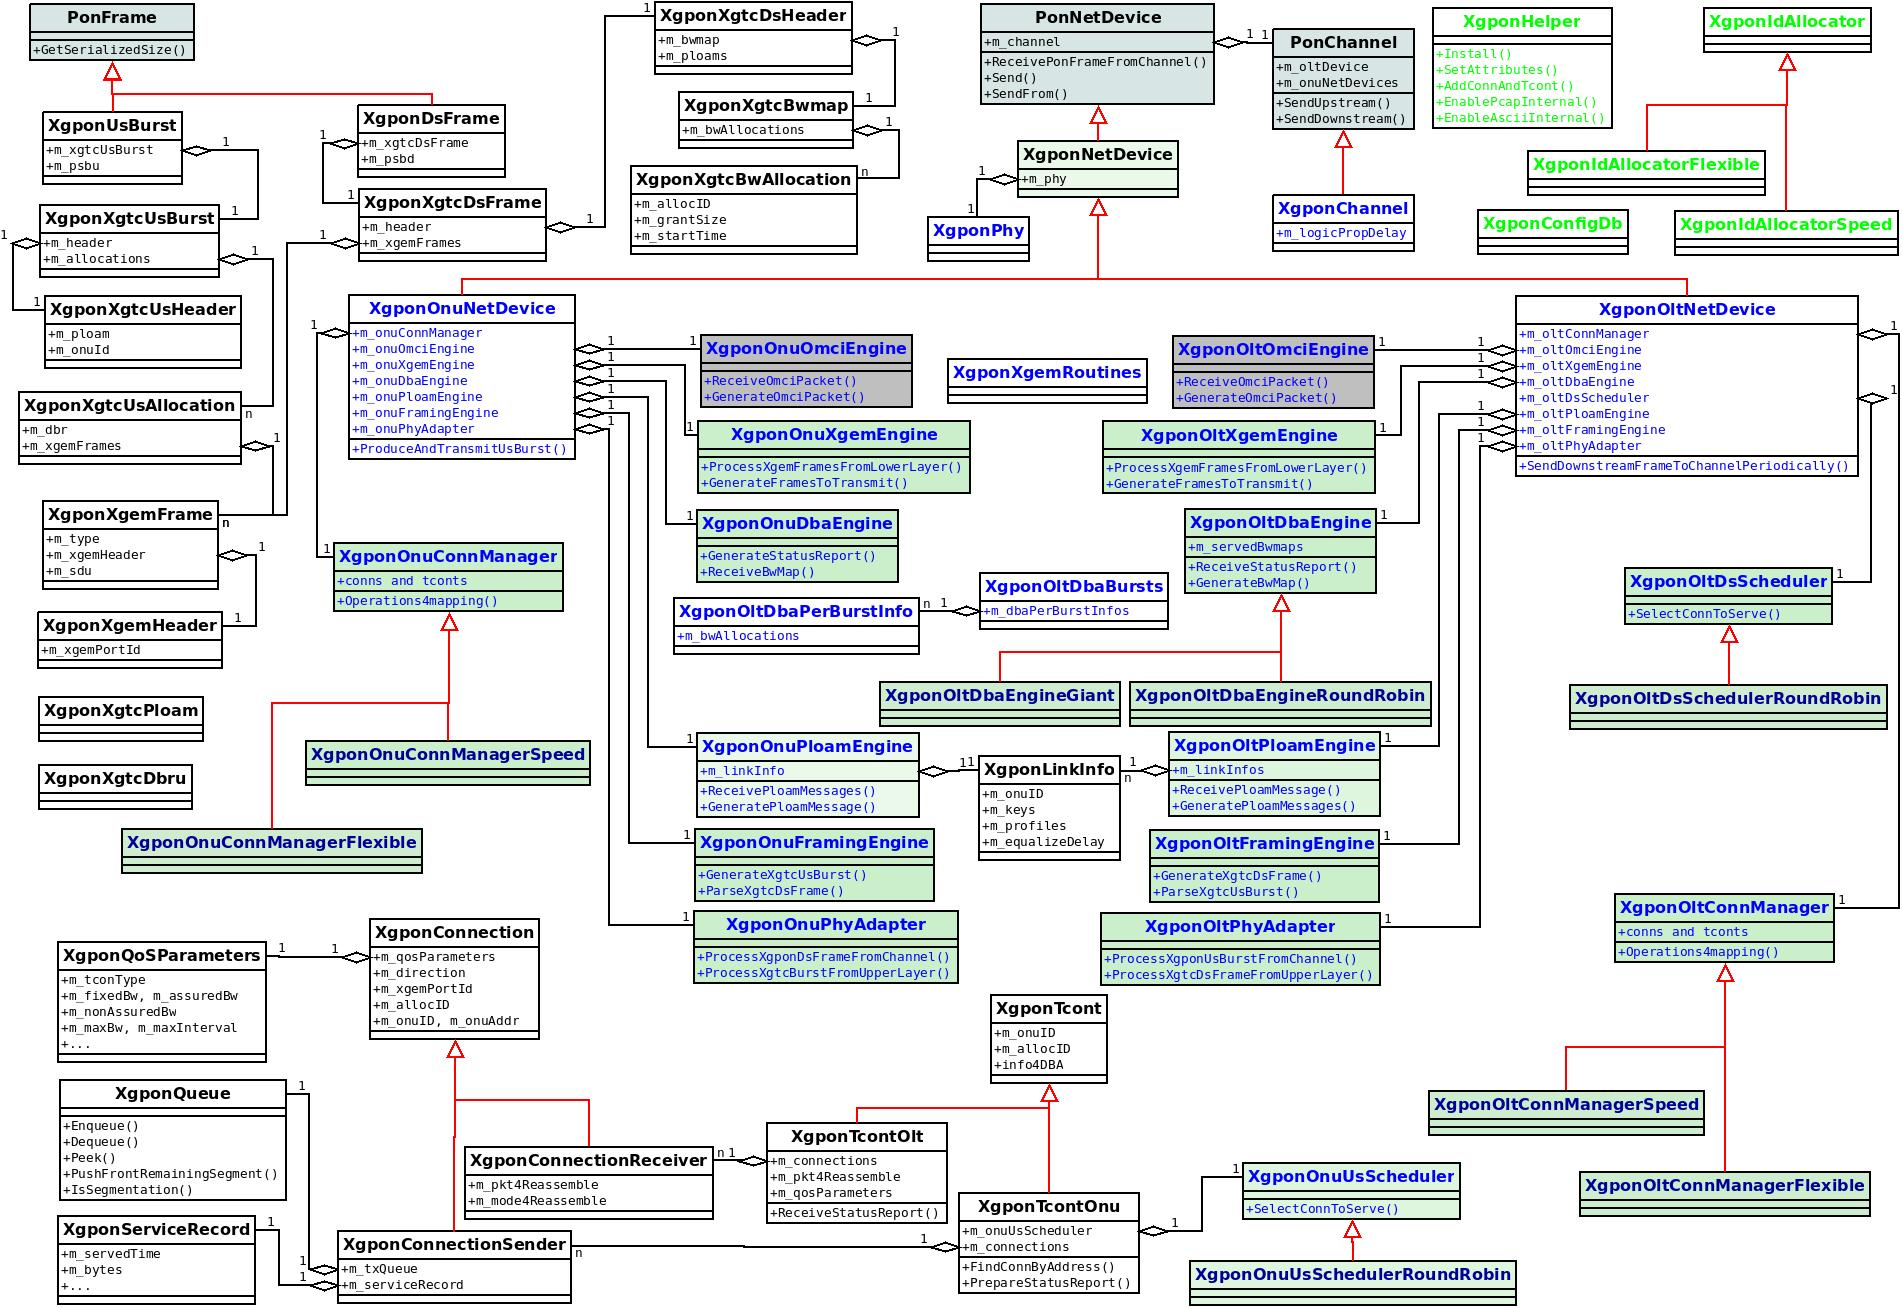
\includegraphics[width=1.4\textwidth]{images/design_classdiagram}
\end{center}
\vspace{-0.1in}
\caption{Class Diagram of the XG-PON module for NS-3}
\label{fig_xgpon_classdiagram}
\end{figure*}

\end{landscape}

\subsection{The Design and Implementation Details}



Figure \ref{fig_xgpon_classdiagram} shows the main classes of this
XG-PON module. Following this class diagram, the design and
implementation details of this module are presented below.

\subsubsection{Channel and Network Devices}

PonChannel and PonNetDevice are the base classes for a general PON
network. Through developing different subclasses, we can simulate
other PON technology (10G-EPON \cite{ieee0910GEPON8023av}, etc.)
and compare with XG-PON. PonChannel is inherited from Channel of
NS-3 and is used to simulate the optical distribution network
(ODN). It has implemented the functions for managing network
devices of the OLT and ONUs attached to this ODN. PonNetDevice is
inherited from NetDevice of NS-3 and is responsible to communicate
with upper layers and PonChannel.


\emph{XgponChannel} is the subclass of PonChannel for XG-PON and
its implementation has been discussed in
\ref{subsection_xgponoverview}. As a subclass of PonNetDevice,
\emph{XgponNetDevice} is used to represent a network device
attached to XgponChannel. It also implements the functions that
are common for both OLT and ONU, such as the statistics for the
network device. XgponOltNetDevice and XgponOnuNetDevice are its
subclasses for the OLT and ONU, respectively. They mainly act as
the container of various engines that implement the protocol stack
of XG-PON.

\subsubsection{Frame Structure}

\emph{PonFrame} represents the frame transmitted over the ODN of a
PON and it just provides the interfaces for (de)serialization,
etc. \emph{XgponDsFrame} and \emph{XgponUsBurst} are used to
represent the downstream frame and the upstream burst of XG-PON,
respectively. There are many other classes used to represent the
related data structures, such as BW$_{map}$, PLOAM message, and
the header of PHY adaptation sublayer (Figure \ref{fig_xgpon_frame_files}). 

\emph{XgponXgemFrame} is used to represent XGEM frame. It includes
the payload (one packet from the upper layer) and one header
defined by XG-PON standard. \emph{XgponXgemHeader} is used to
represent this header of XGEM frame.



\subsubsection{Connection Management}

Since XG-PON traffic is carried by logic connections, many classes
are designed and implemented for representing, organizing, and
handling these connections.

\emph{XgponConnection} is used to represent a connection (XGEM
Port). It mainly contains the identifiers of this connection (XGEM
Port-Id, ONU-ID, etc.). XgponConnectionReceiver and
XgponConnectionSender are its subclasses that represents a
connection at the receiver and sender side.
XgponConnectionReceiver mainly holds the received segments for
reassembling. XgponConnectionSender contains the service history
(XgponServiceRecord), QoS parameters (XgponQosParameters), and the
transmission queue for SDUs from upper layer (XgponQueue).

\emph{XgponTcont} is the class for representing T-CONT.
XgponTcontOnu, its subclass for the ONU, is designed to organize
the upstream connections of the same T-CONT. As for XgponTcontOlt,
the subclass of XgponTcont for the OLT, queue occupancy reports
from ONU, QoS parameters and service history of this T-CONT are
maintained for DBA algorithm. XgponTcontOlt is also responsible to
hold the received segments for implementing reassembly.

\emph{XgponOnuConnManager} contains a list of downstream
connections (XgponConnectionReceiver) and a list of T-CONTs. Note
that each T-CONT might have multiple upstream connections
(XgponConnectionSender). It is also responsible to map SDU/XGEM
frame to the corresponding connection. Thus, it implements both
Downstream Connection Manager and Upstream Connection Manager for
the ONU.

\emph{XgponOltConnManager} is designed to fulfill the functions of
Downstream Connection Manager and Upstream T-CONT Manager for the
OLT. It contains a list of broadcast connections
(XgponConnectionSender). It also contains all uni-cast downstream
connections (XgponConnectionSender) and T-CONTs for upstream
traffic (XgponTcontOlt).

For both XgponOnuConnManager and XgponOltConnManager, we have
implemented several subclasses in which these data structures are
organized in different ways for different purposes.
XgponOnuConnManagerSpeed and XgponOltConnManagerSpeed impose some
relationships among XGEM Port-Id, Alloc-Id, ONU-ID, and IP address
of the computer connected to ONU. They can carry out mapping very
quickly, but they also limit the number of XGEM Ports that one ONU
could have. XgponOnuConnManagerFlexible and
XgponOltConnManagerFlexible don't have such limitations,but they
are much slower. Since millions of packets need to be processed
per second, XgponOnuConnManagerSpeed and XgponOltConnManagerSpeed
should be used for most cases.



\subsubsection{PMD and PHY Adaptation}

PMD Engine and PHY Adaptation Engine in Figure
\ref{fig_xgpon_functionblock} are simplified significantly for
simulating XG-PON with reasonable speed.

\emph{XgponPhy} is used to implement PMD Engine and it mainly
maintains the physical layer parameters that are common for the
OLT and ONUs, such as the downstream data rate and the upstream
data rate of XG-PON. The data rates can be configured through the
attribute system of NS-3. The most important interface is to
tell other classes about the size of one downstream/upstream frame.

\emph{XgponOltPhyAdapter} and \emph{XgponOnuPhyAdapter} are used
to implement PHY Adaptation Engine for the OLT and ONU,
respectively. Instead of simulating their functions (line coding,
FEC, scrambling, etc.) step by step, they just passes
frames/bursts between XgponChannel and Framing Engine after
removed physical layer header. Hence, we implicitly assume that
all frames/bursts can be received correctly. Since the network
should be well planned and FEC has been adopted, the observed
frame corruption rate will be very low and this assumption is
reasonable. In the future, the corruption of frames will be
simulated based on the distance between OLT and ONU or 
empirical measurements of XG-PON networks in real world. 




\subsubsection{Framing Engines}

\emph{XgponOltFramingEngine} implements Framing Engine on the OLT
side. It is responsible to generate the downstream XGTC frames and
parse the upstream XGTC bursts. \emph{XgponOnuFramingEngine}
implements Framing Engine on the ONU side. It is responsible to
generate the upstream XGTC bursts and parse the downstream XGTC
frames. Both of them follow the standard strictly.


\subsubsection{XGEM Engine}
\emph{XgponXgemRoutines} implements some routines that are common
for both the OLT and ONU, such as XGEM frame creation.

As for XGEM Engine functions, they are implemented by
XgponOltXgemEngine and XgponOnuXgemEngine for the OLT and ONU.
They carry out encapsulation, decapsulation, fragmentation,
reassembly, etc. fragmentation and reassembly are implemented
based on the Packet class of NS-3. The logic for data
encryption/decryption is also implemented. But the cryptographic
algorithm is not implemented and executed for saving CPU.

When they are called to produce the payload of a downstream frame
or upstream burst, they will resort Downstream Scheduler or
Upstream Scheduler for determining the traffic to be transmitted.
When getting XGEM frames from Framing Engine, XgponOnuXgemEngine
need extract and only process its own traffic.

\subsubsection{Scheduling and DBA}

To study different scheduling and DBA schemes, several abstract
classes are used in this module for extensibility. The actual
schedulers can then inherit these abstractions and implement their
specific algorithms. The related classes in this module are
introduced below.

\emph{XgponOltDsScheduler} acts as the OLT Downstream Scheduler
shown in Figure \ref{fig_xgpon_functionblock}. When
XgponOltXgemEngine generates the payload of a downstream XGTC
frame, it will call one virtual function of XgponOltDsScheduler
(\emph{SelectConnToServe}) to decide the connection to be served.
XgponOltSimpleDsScheduler is one subclass that follows the round
robin scheme.

\emph{XgponOltDbaEngine} is designed for the OLT DBA Engine shown
in Figure \ref{fig_xgpon_functionblock}. When
XgponOltFramingEngine generates one downstream XGTC frame, it will
resort XgponOltDbaEngine to generate a BW$_{map}$. XgponOltDbaEngine 
is also responsible to receive queue occupancy reports from ONUs. 
Currently, a simple DBA algorithm is implemented in 
XgponOltDbaEngineRoundRobin that serves a fixed amount of bytes 
for each T-CONT in a round robin manner. GiantMAC \cite{leligou06GiantMACforGPON}
has also been implemented in XgponOltDbaEngineGiant for supporting different
kinds of T-CONTs with various QoS parameters.


\emph{XgponOnuDbaEngine} acts as the ONU DBA Engine shown in
Figure \ref{fig_xgpon_functionblock}. It is responsible to process
BW$_{map}$, generate queue occupancy report, and schedule to
generate and transmit the upstream burst.

\emph{XgponOnuUsScheduler} acts as the ONU upstream scheduler
shown in Figure \ref{fig_xgpon_functionblock}. When
XgponOnuXgemEngine generates the payload of one upstream burst,
XgponOnuUsScheduler is resorted to decide the connections to be
served in the transmission opportunity assigned to one T-CONT.
XgponOnuUsSchedulerRoundRobin is one subclass implemented to serve
the connections of one T-CONT in a round robin manner. Note that
XgponOnuUsScheduler is put within XgponTcontOnu so that T-CONTs of
the same ONU may use different scheduling algorithms for their
upstream traffic.



\subsubsection{Miscellaneous}

\emph{XgponOltPloamEngine} and \emph{XgponOnuPloamEngine} are
designed for exchanging Ploam messages between the OLT and ONU.
They also uses \emph{XgponLinkInfo} to maintain per-ONU
information, such as keys and burst profiles. As for
\emph{XgponOltOmciEngine} and \emph{XgponOnuOmciEngine}, they are
designed for implementing the OMCI channel. For these classes, we
have just implemented their interactions with other classes of
this module. We will simulate their messages and  the related
procedures in the future.


\subsubsection{Helper}

For facilitating researchers to configure one XG-PON network with
hundreds of ONUs and thousands of connections, \emph{XgponHelper}
is also implemented in this module. Through XgponHelper,
researchers can install XgponNetDevice on nodes and attach them to
XgponChannel. They can also configure XGEM Ports and T-CONTs for
carrying user traffic. Researchers can also use XgponHelper to
enable Ascii and Pcap tracing.

\emph{XgponConfigDb} is one database that holds the information
used by XgponHelper. Before using XgponHelper, researchers should
first configure subclasses and parameters used in the simulation.
When adding XGEM Port/T-CONT/ONU into XG-PON,
\emph{XgponIdAllocator} is used to get the corresponding XGEM
Port-Id/Alloc-Id/ONU-ID. \emph{XgponIdAllocatorSpeed} is the
subclass developed for imposing some relationship among XGEM
Port-Id, Alloc-Id, ONU-ID, and IP address of the node connected to
ONU with aim of speeding up XG-PON simulation. XgponConfigDb uses
one flag to make sure that XgponOltConnManagerSpeed,
XgponOnuConnManagerSpeed, and XgponIdAllocatorSpeed are used
together.
